\subsection{Backend}

O desenvolvimento do \textit{backend} constituiu uma das partes fundamentais do projeto, assegurando a implementação da lógica de negócio, a gestão dos dados e a comunicação entre o sistema e a interface de utilizador. Este componente atua como a camada central responsável por garantir que os processos internos sejam executados de forma consistente, segura e eficiente, proporcionando suporte às funcionalidades disponibilizadas no \textit{frontend}.  

Nesta secção irá se apresentar funcionalidades do backend no contexto da US3 (definida na tabela \ref{tab:req-funcionais}).

\subsubsection{Spring}

A framework Spring apresentou à equipa uma alta curva de aprendizagem. Os vários conceitos e ferramentas nesta são bastante alienígenas a qualquer outra ferramenta antes utilizada pelos membros. Por tal foi necessário mais tempo para a aprender. Alguns dos conceitos-chave considerados incluem:

\begin{itemize}
    \item \textbf{\textit{Spring Data}} é um agregado de módulos Spring que têm como função principal facilitar a programção de entidades e o seu respetivos acesso quando conectado a uma fonte de dados.
    \item \textbf{\textit{Spring Data JPA}} (ou só \textit{JPA}) é um dos módulos pertencente à coletânea Spring Data. O seu objetivo é facilitar a implementação de repositórios, reduzindo estes a interfaces Java, nas quais o Spring analisa o nome do método e implementa em \textit{runtime} o mesmo. 
    \item \textbf{\gls{Hibernate}} \cite{docs-hibernate} é uma framework Java e uma solução \ACRshort{ORM} que serve como implementação do \textit{JPA} para, logicamente, persistir a informação na respetiva base de dados.
\end{itemize}

\subsubsection{Estrutura de pastas}

A estrutura de pastas do backend foi definida para enaltecer a função de cada ficheiro e/ou classe em cada uma, como pode ser observado na figura \ref{fig:folder-struct-backend}.

\begin{figure}
    \centering
    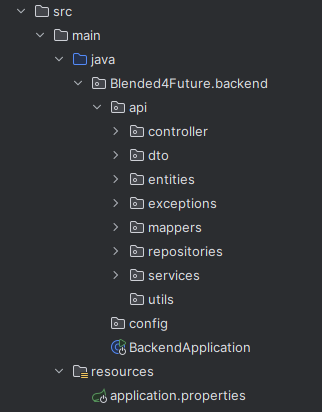
\includegraphics[width=0.5\linewidth]{capitulos/cap4-implementacao/assets/fold-struct-backend.png}
    \caption{Estrutura de pastas do backend}
    \label{fig:folder-struct-backend}
\end{figure}

\subsubsection{Entidades e relações}

Para o caso de uso a ser considerado, a entidade de maior importância será \textit{Project}. Esta encontra-se representada na figura \ref{fig:classe-projeto}.

Em nota, interessante enaltecer o uso das respetivas anotações:

\begin{itemize}
    \item \textbf{\textit{@Entity}} informa o \ACRshort{JPA}/\gls{Hibernate} que esta é uma entidade que deve ser persistida. Para tal deve conter um argumento anotado \lstinline|@Id|.
    \item \textbf{\textit{@Data}}\cite{docs-annotation-data} serve como substituto para as anotações \lstinline|@ToString|, \lstinline|@EqualsAndHashCode|, \lstinline|@Getter|, \lstinline|@Setter| e \lstinline|@RequiredArgsConstructor| que, respetivamente: 
    
    \begin{itemize}
        \item implementa o método \lstinline|toString()| incluindo todos os parâmetros não estáticos da classe;
        \item implementa o método \lstinline|equals(Object object)| e \lstinline|hashCodeO()|. Uma definição (\lstinline|callSuper|) teve de ser subscrita, pois era desejado inclusão dos atributos da superclasse \lstinline|BaseEntity| neste método (ver secção \ref{sec:base-entity});
        \item implementa métodos \textit{getter} para todos os atributos privados
        \item implementa metodos \textit{setter} para todos os atributos privados
        \item implementa um construtor com um parâmetro por atributo não final da classe.
    \end{itemize}

\end{itemize}


\begin{figure}
    \centering
    
    \begin{lstlisting}[language=Java]

@Entity
@Data
@EqualsAndHashCode(callSuper = true)
public class Project extends BaseEntity {

    @Column(nullable = false)
    @Convert(converter = ProjectName.NameConverter.class)
    private ProjectName name = new ProjectName();

    @Column(nullable = false)
    @Convert(converter = ProjectDescription.DescriptionConverter.class)
    private ProjectDescription description = new ProjectDescription();

    @ManyToOne
    private Company company;

    @ManyToOne
    private CompanyRepresentative companyRepresentative;

    @ManyToMany
    private Set<Student> students = Set.of();

    @ManyToMany
    private Set<Qualification> qualifications = Set.of();

    @OneToMany(mappedBy = "project", cascade = CascadeType.REMOVE)
    private Set<Report> reports = Set.of();

    @ManyToOne
    private CourseEdition courseEdition;
}

    \end{lstlisting}

    \caption{Classe \textit{Project}}
    \label{fig:classe-projeto}
\end{figure}

\subsubsection{\textit{BaseEntity}}
\label{sec:base-entity}

Como medida de segurança e de padronização, foi desenvolvida a classe \textit{BaseEntity} (ver listagem \ref{lst:base-entity}). Esta classe define dois identificadores: um interno e um externo. O identificador externo é utilizado na comunicação com o cliente, sendo retornado nos pedidos sob a forma de \textit{DTO}, enquanto o identificador interno é reservado para uso exclusivo do sistema.

Tal como o próprio nome indica, a \textit{BaseEntity} foi concebida para servir como \textit{superclasse} de todas as entidades persistentes.

A implementação da \textit{BaseEntity} envolve várias decisões de \textit{design} que merecem atenção:

\begin{itemize}
    \item No \gls{Hibernate}, os atributos definidos em superclasses não são, por defeito, persistidos. A utilização da anotação \lstinline|@MappedSuperclass| assegura que as classes filhas possam herdar esses parâmetros, permitindo a sua correta persistência na base de dados.

    \item A anotação \lstinline|@Id| define o atributo \lstinline|iid| como identificador principal da entidade no contexto da persistência. Complementarmente, \lstinline|@GeneratedValue(strategy=GenerationType.UUID)| especifica a forma como o identificador deve ser gerado, recorrendo ao padrão \textit{UUID}. Esta opção é particularmente relevante dado que, por omissão, o \gls{Hibernate} apenas consegue popular atributos de tipos primitivos.
    
    \item Verificou-se a necessidade de avaliar, de forma global, todos os atributos relacionados com a lógica de negócio, de modo a identificar e retornar eventuais erros existentes. Para esse fim, a função \lstinline|isBusinessDataValid()| analisa todos os \textit{Value Objects} (Ver secção \ref{sec:backend-value-objects}) da respetiva classe e devolve um \lstinline|HashMap| contendo a listagem dos erros detetados.
\end{itemize}

\begin{lstlisting}[language=Java,caption={Classe \textit{BaseEntity}},label={lst:base-entity}]
@MappedSuperclass
@Getter
public abstract class BaseEntity {

    /**
     * This field is the internal identifier for the entity.
     * It is used for database operations and should not be exposed in API responses.
     * @summary iid = Internal Identifier
     */
    @Id
    @GeneratedValue(strategy = GenerationType.UUID)
    private UUID iid;

    /**
     * This field is the external identifier for the entity.
     * This is the one that should be used in API responses and requests.
     * @summary eid = External Identifier
     */
    @Column(name="eid", unique = true, nullable = false)
    private UUID externalId;

    public BaseEntity() {
        this.externalId = generateCode();
    }

    private UUID generateCode() {
        return UUID.randomUUID();
    }

    public HashMap<String, Object> isBusinessDataValid() {

        HashMap<String, Object> errors = new HashMap<>();

        Class<?> clazz = this.getClass();
        List<IValueObject<?>> valueObjects = new ArrayList<>();

        while (clazz != null && clazz != Object.class) {
            for (Field field : clazz.getDeclaredFields()) {
                field.setAccessible(true);
                try {
                    Object value = field.get(this);

                    if (value instanceof IValueObject<?> vo) {
                        valueObjects.add(vo);
                    }
                } catch (IllegalAccessException ignored) {}
            }
            clazz = clazz.getSuperclass();
        }

        return isBusinessDataValid(valueObjects);
    }

    public static HashMap<String, Object> isBusinessDataValid(List<IValueObject<?>> fields) {
        HashMap<String, Object> errors = new HashMap<>();
        for (IValueObject<?> field : fields) {
            if (field == null) {
                continue;
            }
            errors.putAll(field.isValid());
        }
        return errors;
    }
}

\end{lstlisting}




\subsubsection{\textit{Value Objects}}
\label{sec:backend-value-objects}

A utilização de \textit{Value Objects} permite um maior controlo sobre a lógica de negócio inerente ao projeto. Por tal a sua implementação é necessária aquando a construção de um sistema de superior complexidade. 

A listagem \ref{lst:interface-value-object} mostra a interface \lstinline|ValueObject|.

\begin{lstlisting}[language=Java,caption={Interface \textit{Value Object}},label={lst:interface-value-object}]
public interface IValueObject<T> {
    T getValue();
    public HashMap<String, Object> isValid();
}
\end{lstlisting}

A notar, a função \lstinline|isValid()| em conjunto com a superclasse \lstinline|BaseEntity| permite verificar a lógica de negócio de cada respetivo \lstinline|ValueObject|. Para tal basta implementação fazer uma verificação do objecto em questão e retornar um \lstinline|HashMap| com toda a informação de erros.

\begin{lstlisting}[language=Java,caption={Classe \textit{ProjectDescription}},label={lst:class-project-description}]
@Value
public class ProjectDescription implements IValueObject<String> {

    public static final int MIN_LENGTH = 10;
    public static final int MAX_LENGTH = 500;
    public static final String DEFAULT_DESCRIPTION = "Default Project Description";

    private String description;

    @Override
    public String getValue() {
        return this.description;
    }

    public ProjectDescription(String value) {
        this.description = value;
    }

    public ProjectDescription() {
        this(DEFAULT_DESCRIPTION);
    }

    @Override
    public HashMap<String, Object> isValid() {
        HashMap<String, Object> errors = new HashMap<>();
        if (this.getValue() == null || this.getValue().isEmpty()) {
            errors.put("description", "Description cannot be null or empty");
        } else if (this.getValue().length() < MIN_LENGTH || this.getValue().length() > MAX_LENGTH) {
            errors.put("description", "Description must be between 10 and 500 characters long");
        }
        return errors;
    }

    @Converter
    public static class DescriptionConverter implements jakarta.persistence.AttributeConverter<ProjectDescription, String> {
        @Override
        public String convertToDatabaseColumn(ProjectDescription description) {
            return description.getValue();
        }

        @Override
        public ProjectDescription convertToEntityAttribute(String dbData) {
            return new ProjectDescription(dbData);
        }
    }
}
\end{lstlisting}

A listagem \ref{lst:class-project-description} demonstra uma implementação de \lstinline|IValueObject|. Como referido a função \lstinline|isValid()| avalia se o objeto é valido ou não retornando quaisquer erros.

Importante também seria referir a necessidade de um conversor, uma classe que informa o \gls{Hibernate} como deve mapear o objeto do programa para a base de dados e vice-versa.

\subsubsection{Repositórios}



\subsubsection{Controladores e prevenção de erros}